\documentclass{article}

\usepackage{graphicx}
\usepackage{color}
\usepackage{listings}
\usepackage{amsmath}
\usepackage{amssymb}

\lstset{tabsize=2}

\begin{document}

\title{Q-Learning with Polynomial Approximation Functions}
\author{Graham Northup}
\date{\today}
\maketitle

\begin{abstract}
	Q-Learning, while provably optimal for any Markov process with an
	admissible reward heuristic, suffers from at least exponential state blowup
	with respect to the domains of the feature elements. A simplification is
	proposed herein which allows the state to be approximated by
	arbitrary-degree polynomials, vastly reducing memory requirements, at the
	potential cost of some accuracy in determining the reward heuristic.
	Drawbacks of the algorithm are mentioned, and a practical demonstration is
	given.
\end{abstract}

\section{Basis}

\subsection{Basic Q-Learning}

	Q-Learning is a reinforcement learning (RL) method; as with other RL
	methods, the problem to solve is as follows: given an agent which makes
	limited observations about its environment, which has discrete choices of
	actions to perform at suitable time quanta, and which is aware of the
	relative success their actions have imparted on them, is it possible to
	maximize agent's success (given, e.g., an instance of the environment)?

	\begin{figure}[b]
		\caption{Data flow in an RL problem.}
		\centering
		\def\svgwidth{8cm}
		\input{rl_agent.pdf_tex}
	\end{figure}

	The key observation in Q-Learning is the existence of a {\it heuristic
	function} $Q$ which predicts the expected value of the sum of all future
	rewards starting at this state. In formal definition, given $\vec{F}$ as
	the set of all possible {\it feature vectors}---each of which contains the
	values of all observations---and a set of actions $A$:

	$$
	Q: \vec{F} \times A \rightarrow \mathbb{R}.
	$$

	To preserve boundedness (as the sequence of rewards is permitted not to
	converge), the codomain of this function is usually interpreted as a mean
	with exponentially-decaying weight.

	$Q$ starts as a hidden or unknown function, initialized usually to random
	values; as a simulation progresses, $Q$ is updated by

	$$
	Q_{t+1}(s_t,a_t) = Q_t(s_t,a_t) + \eta ( r_{t+1} + \gamma \operatorname{max}_a Q(s_{t+1},a) - Q_t(s_t,a_t) ).
	$$

	The outer grouping is a simple linear interpolation between the previous
	$Q_t(s_t,a_t)$ and the new value parameterized by $\eta \in [0, 1]$, the
	learning rate; the new value is determined as a linear combination of the
	current reward $r_{t+1}$ (for the action performed at time $t$) and the
	estimated possible maximum reward attainable for all actions $a \in A$
	attainable from the current state $s_{t+1}$, parameterized by $\gamma \geq
	0$. $\gamma$ is the ``discount factor'', which determines how willing the
	agent is to discount actions at the current step for future promised
	rewards---assuming that $Q$ is accurate. $\gamma = 0$ gives a
	``short-sighted'', ``greedy'' agent which always prefers the maximum immediate
	reward, whereas $\gamma$ greater than the maximum of the reward domain will
	give an agent that trusts $Q$ blindly to lead to the absolute maximum
	reward.

	Finally, the actual policy we derive is simple: maximize $Q$:

	$$
	a_{t+1} = \operatorname{argmax}_a Q(s_{t+1}, a).
	$$

	Issues with this formulation are apparent; assume, again, that $\vec{F}$ is
	the set of all feature vectors. We can then assume that, for each $\vec{f}
	\in \vec{F}$, if $f_i \in F_i$, then the size of $\vec{F}$ can be computed
	as

	$$
	\prod_i \|F_i\|.
	$$

	Assume $\|F\| = n$ and that each $\|F_i\|$ is bound below by 2 (as a unary
	observation would be trivial); then it is clear that $\|\vec{F}\| \in
	\Omega(2^n)$, which requires strictly exponential space in terms of the
	number of elements in the feature vector\footnote{Note that we consider
	$\|A\|$ to be a constant factor, and that this discourse does not concern
	issues arising from large $A$.}.

\subsection{Polynomial Approximations}

	Instead of determining the value of $Q$ for {\it every} observation in
	$\vec{F}$, a simple, practical assumption is that certain elements in each
	feature vector $\vec{f}$ {\it correspond}, in some way, to an optimal
	action, usually without regard to the specifics of other features. While
	there are many ways to approximate this correspondence, we operate under
	the assumption that, in our case, features are selected such that a
	polynomial of degree $d$ may be used to approximate the relevancy of a
	given action for a given feature. As is traditional, we assume that the
	initial coefficients of the polynomial are initialized at random, and
	revise the definition and update of the $Q$ function as follows:

	$$
	Q: \mathbb{Z}_{\|F\|} \times A \rightarrow \mathbb{R}^d,
	$$

	$$
	Q_{t+1}(f,a_t)_i = Q_t(f,a_t)_i + \eta \Gamma^i ( r_{t+1} + \gamma \operatorname{max}_a Q(f,a)_i - Q_t(f,a_t)_i ).
	$$

	The variable $f$ now represents not the vector, but the index of the
	feature instead. The new variable, $\Gamma \in (0, 1]$, is used to give an
	exponentially growing discount for successively higher powers; this serves
	the dual role of ensuring that rewards don't unduly increase high-power
	terms, and causing the higher powers to follow a time-based,
	exponentially-weighted mean of the lower powers\footnote{Note that this
	comes at the price of losing a sane interpretation of terms $i \geq 1$; for
	$i = 0$, the value is, as it was in the original Q-Learning algorithm, the
	expected value of the sum of all rewards for the optimal path from the
	given state after the given action.}.

	The evaluation of the policy must also change ever so slightly to
	accomodate the approximation polynomial:
	$$
	a_{t+1} = \operatorname{argmax}_a \sum_i  Q(f,a)_i s_{t}^i,
	$$
	where it should be clear that the inner sum is merely the evaluation of a
	polynomial with coefficients $Q(f,a)$ on the feature element $s_t = \vec{f}_f$.

	Finally, as an added consideration, and because of the expected error in
	the approximation, it is helpful to ``forget'' invalid information caused by
	unusual circumstances over time. While this is optional, our implementation
	includes a decay factor $\epsilon \in (0, 1]$ which is multiplied into
	every element after an episode:

	$$
	Q_{t+1}(f,a_t)_i = \epsilon Q_t(f,a_t)_i.
	$$

	The most important concern we had prior was the memory size; hopefully it
	is clear that, since we don't intend to update $Q$ for all possible {\it
	values} in the feature vector---instead, the feature vector indices
	suffice. The memory requirements are therefore bounded by $\Theta(nd)$,
	which is far better than $\Omega(2^n)$.

\section{SneqBot: An Implementation}

	The practical demonstration of this learning algorithm is SneqBot, an agent
	for playing Slither.io\footnote{http://slither.io/}. The code is attached,
	but listings will be included here. Slither.io is an effective
	demonstration of RL agents for a variety of reasons:

	\begin{itemize}
		\item It operates in real-time---unlike many other RL agent
			simulations, the time scale {\it is} attached to the current real
			time.
		\item It has a scoring system which is directly tied to the reward
			system.
		\item It is played against human players who involve themselves with a
			great deal of strategy.
		\item It uses a thin-client model; the client is sent exactly enough
			information to render the current game state, and sends back only
			controls. Simulation happens on a server out of reach of the
			clients themselves, so the agents can't ``cheat''.
		\item The game is written in JavaScript, which opens it immediately to
			a wide array of debuggers, editors, extensions, and other utilities
			for inspecting, modifying, and changing the game state.
		\item It has a definite (if undesirable) end state which marks the end
			of an episode.
		\item The ``inputs'' to the game consist almost exclusively of an angle
			and a single boolean (heading and accelerating).
	\end{itemize}

	\begin{figure}[!b]
		\caption{A typical state of Slither.io. The player-controlled snake is the one with its head in the center of the viewport.}
		\centering
		
\includegraphics[width=8cm]{slither_io.png}
	\end{figure}

	Slither.io has a play field that is 40000 by 40000 units, with an inscribed
	circle describing the border. The player (or agent) controls a snake which,
	like the original game of snake, finds and eats food, and grows as a
	result. Unlike the original game, however, the player's own snake can
	intersect with itself. Furthermore, as mentioned previously, the game is
	multiplayer; one ``loses'' by colliding with another player's snake, or the
	field's border. Upon death by colliding with another snake, the outline of
	the snake turns into very dense food, which incentivizes the destruction of
	other players to gain food\footnote{No food is dropped when colliding with
	the field border.}.

	We observed the strategies of human players; while they are varied, the
	most successful strategies make use of a technique we call ``constriction'',
	wherein one player entirely surrounds another player. Care must be taken to
	avoid the constrictor from running into the constricted player, but,
	inevitably, due to interpolation between points on the snake's lengths,
	loops subtended by snakes eventually become smaller and smaller (and have
	been observed to be singular at times), thus eventually guaranteeing that
	the constricted snake would collide with the constrictor and die.
	
	To make Q-Learning effective, we needed to set up a feature vector over
	which it could be theorized that the optimum policy would be attainable by
	maximizing or minimizing the values of polynomials evaluated over its
	elements. Empirically, we chose the following elements:

	\begin{enumerate}
		\setcounter{enumi}{-1}
		\item Distance to the field's center ($(20000, 20000)$), normalized by
			the field's radius ($20000$).
		\item Distance to the nearest food, normalized by the field radius.
		\item Size of the nearest food (in arbitrary units, bounded
			aproximately above by 10).
		\item Distance to the nearest snake, normalized by the field radius.
		\item Size of the nearest snake (in arbitrary units; bound below by 1,
			the largest snakes would grow to perhaps 30-40).
		\item Number of snakes actually visible (though not necessarily always
			seen within the browser's viewport).
		\item Occluded solid angle of some number of raycasts from the player
			snake's head, $[0, 1]$. Calculation of this value also created an
			``escape vector'', a direction toward the least occluded path, as
			needed to escape a possible constriction.
	\end{enumerate}

	These values are generated by the {\tt STATE\_FUNCTIONS}, an array of
	niladic functions which return objects whose {\tt ``st''} property is an
	array which will be concatenated into the final feature vector. Note that
	there's no correspondence between the number of {\tt STATE\_FUNCTIONS} and
	the elements of the feature vector; thus the variable {\tt
	STATE\_CARDINALITY} exists to instruct the learner of the size of the
	feature vector. We also found it important to normalize some of these
	features---for example, the distance from the center can be at most 20000,
	while the size of a food item is rarely greater than 10, and so learning
	updates would consider distance from the center several orders of magnitude
	``more important'' than food size for even trivial variations in the reward
	function. The {\tt STATE\_FUNCTIONS} used by SneqBot are given in Appendix
	A.

	The actions which can be undertaken are described in {\tt
	ACTION\_FUNCTIONS}, which contains unadic functions whose single argument
	is the data array generated by mapping all {\tt STATE\_FUNCTIONS} through
	the application operator. From these values, the action functions receive
	additional data from the state functions, such as the actual location of
	the nearest food (passed as additional properties of the objects returned
	by the state functions). In this way, the action functions avoid doing work
	twice, and are permitted to operate at a reasonably high level of
	abstraction---such as ``move toward nearest food'' or ``cut off nearest
	snake''. This array is given in Appendix B.

	The actual learner is defined in {\tt q.js}, along with its polynomial
	approximation. Key parts of the learning algorithm are as follows: the $\{a
	| Q(s, a)\}$ evaluator:

	\begin{lstlisting}
eval(states) {
	var max_pow = this.max_pow;
	var weights = this.state_norm;
	states = states.map((v, idx) => v * weights[idx]);
	return this.heur.map(weights => 
		weights.map((poly, idx) =>
			eval_poly(poly, states[idx], max_pow)
		).reduce((a, b) => a + b, 0)
	);
}
	\end{lstlisting}

	The policy function:

	\begin{lstlisting}
getBestAction(states) {
	if(Math.random() < this.noise) {
		return Math.floor(this.n_act * Math.random());
	}
	var prios = this.eval(states);
	return argmax(prios)[0];
}
	\end{lstlisting}

	The value update function:

	\begin{lstlisting}
cumulateReward(states, act, reward) {
	reward *= this.reward_scale;
	var weights = this.state_norm;
	states = states.map((v, idx) => v * weights[idx]);
	for(var st = 0; st < this.n_state; st++) {
		for(var i = this.min_pow; i <= this.max_pow; i++) {
			this.heur[act][st][i - this.min_pow] += 
				reward * states[st] * this.eta * Math.pow(this.gamma, i);
		}
	}
}
	\end{lstlisting}

	The decay step:

	\begin{lstlisting}
decayAll() {
	for(var act = 0; act < this.n_act; act++) {
		for(var st = 0; st < this.n_state; st++) {
			for(var pow = this.min_pow; pow <= this.max_pow; pow++) {
				this.heur[act][st][pow - this.min_pow] *= this.decay;
			}
		}
	}
}
	\end{lstlisting}

	And, lastly, the constructor for a {\tt Learner}, with all default values
	we used for the demonstration:

	\begin{lstlisting}
constructor(n_act, n_state, min_pow, max_pow, key) {
	if(min_pow == undefined) min_pow = -2;
	if(max_pow == undefined) max_pow = 2;
	if(key == undefined) key = "";
	this.n_act = n_act;
	this.n_state = n_state;
	this.min_pow = min_pow;
	this.max_pow = max_pow;
	this.gamma = 0.15;
	this.eta = 0.5;
	this.decay = 0.99;
	this.noise = 0.02;
	this.reward_scale = 1;
	this.key = key;
	this.state_norm = (new Array(this.n_state)).map(() => 1);
	this.loadHeuristic();
}
	\end{lstlisting}

	Finally, the actual reward function and main loop ran a slightly
	desynchronized schedule; SneqBot was instructed to ``think'' about its
	actions once every 15ms (or at about 60Hz), and evaluated all state,
	policy, and the best action at that rate. Every 500mS (2Hz), SneqBot would
	``learn'' by comparing its current length to its previous length. Code for
	both sections is given in Appendix C.

	While the basis of all rewards is simply the change in length (or,
	equivalently, the change in score), some additional adjustments were made
	to attempt to improve SneqBot's performance and reduce needless behavior.
	For example, a small negative bias was added to the computation of length
	change; if no significant changes occurred to the snake's length, SneqBot
	would therefore be discouraged from that behavior (and more motivated to
	attempt an effective strategy). Similarly, SneqBot was rewarded slightly
	for being in an area free of other snakes, as we observed that the other
	(human) players were the most obvious threat to SneqBot. Finally, at the
	end of an episode (when the controlled snake dies), we significantly
	penalize the choice of action that led to SneqBot's demise.

\section{Results}

	We were unable to acquire enough data to be certain that the modified
	Q-Learning algorithm would work in practice; however, SneqBot is indeed
	based on an earlier attempt (called ``SnekBot'') which used polynomial
	approximations of state (but no learning algorithm---all online learning
	was done by the user), and which could play at a ``reasonably mediocre''
	level---not enough to fend off a directed attack by a human, but certainly
	enough to reach the average score attained by novices. While we would have
	liked to verify that SneqBot could learn parameters allowing it to play
	competitively with SnekBot (and perhaps even surpass it), our current
	results remain inconclusive.

	Much future work is possible; while working on SneqBot, we experimented
	with the use of rational polynomial approximators, but abandoned the idea
	due to various conceptual issues (e.g., the singularities experienced by
	rational functions as their divisors approach 0). We also would have liked
	to have the learning update of SneqBot update certain input parameters used
	for its actual feature detection---for example, so that it could learn the
	optimal ratio of food size to distance, so that it might seek larger food
	even if it is not the closest (such features were, in fact, already
	implemented in the predecessor SnekBot, but, again, SnekBot has no learning
	apparatus).

	\begin{figure}[b]
		\caption{A snek (or sneq).}
		\centering
		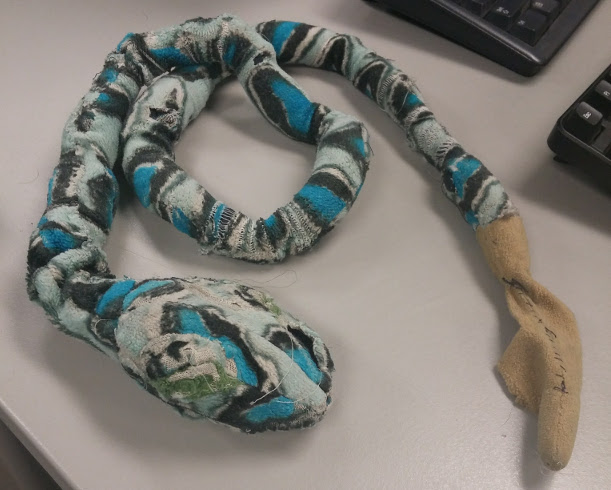
\includegraphics[height=5cm]{snek.jpg}
	\end{figure}

\section{Appendices}

\subsection{Appendix A}

	\begin{lstlisting}
/***** STATE FUNCTIONS *****/

var STATE_FUNCTIONS = [
	() => {
		return {"type": "center", "st": [norm(snake.xx, snake.yy, 2e4, 2e4)]};
	},
	() => {
		var fpts = [];
		foreach_food((x, y, sz, fd) => fpts.push({"norm": norm(x, y, snake.xx, snake.yy), "x": x, "y": y, "sz": sz}));
		fpts.sort((a, b) => a.norm - b.norm);
		var fpt = fpts[0];
		dbgctx.strokeStyle = "#0f0";
		dbg_drawpt(fpt.x, fpt.y);
		return {"type": "food", "st": [fpt.norm, fpt.sz], "food": fpt};
	},
	() => {
		var closestpt = null, closestnorm = -1, closestsn = null;
		foreach_snek_pt((px, py, snek, sni, ipt) => {
			var sr = snek.sc * SIZE_TO_RADIUS;
			if(ipt == snek.pts.length - 1) sr *= HEAD_INFLATE;
			if(closestpt == null || (norm(snake.xx, snake.yy, px, py) - sr) < closestnorm) {
				closestpt = [px, py];
				closestnorm = norm(snake.xx, snake.yy, px, py);
				closestsn = snek;
			}
		});
		var pris = [4e4, 0, 0, 4e4, 4e4, 4e4];
		if(closestpt != null) {
			pris[0] = closestnorm;
			pris[1] = closestsn.sc;
			pris[2] = (closestsn.ang + snake.ang) % TAU;
			var headpt = closestsn.pts[closestsn.pts.length - 1];
			pris[3] = norm(headpt.xx, headpt.yy, snake.xx, snake.yy);
			var fwdpt = [headpt.xx + closestsn.sp * Math.cos(closestsn.ang), headpt.yy + closestsn.sp * Math.sin(closestsn.ang)];
			var sr = closestsn.sc * SIZE_TO_RADIUS;
			var dx = fwdpt[0] - headpt.xx, dy = fwdpt[1] - headpt.yy;
			var cutoff_t = closest_on_line(headpt.xx, headpt.yy, fwdpt[0], fwdpt[1], snake.xx, snake.yy)[2];
			var dist = norm(0, 0, dx, dy);
			cutoff_t += LEAD_FACTOR * (sr / dist);
			var cutoff = [headpt.xx + dx * cutoff_t, headpt.yy + dy * cutoff_t];
			pris[4] = norm(cutoff[0], cutoff[1], headpt.xx, headpt.yy) / (dist * closestsn.sp);
			pris[5] = norm(cutoff[0], cutoff[1], snake.xx, snake.yy) / (dist * snake.sp);
			dbgctx.strokeStyle="#f0f";
			dbg_drawpt(closestpt[0], closestpt[1], 25);
			dbgctx.strokeStyle="#ff0";
			dbg_drawpt(cutoff[0], cutoff[1], 25);
		}
		return {"type": "snake", "st": pris, "snek": closestsn, "snekpt": closestpt, "cutoff": cutoff};
	},
	() => {
		return {"type": "snake_count", "st": [snakes.length]};
	},
	() => {
		var snpts = [];
		foreach_snek_pt((px, py, snek, sni, ipt) => snpts.push([px, py, snek.sc * SIZE_TO_RADIUS]));
		var ang_hits = {};
		var num_hits = 0;
		dbgctx.strokeStyle = "rgba(255, 0, 0, 63)";
		for(var theta = 0; theta < TAU; theta += SA_RESOLUTION) {
			var hit = false;
			var ex = snake.xx + SA_LENGTH * Math.cos(theta);
			var ey = snake.yy + SA_LENGTH * Math.sin(theta);
			for(var ipt = 0; ipt < snpts.length; ipt++) {
				var pt = snpts[ipt];
				var pts = seg_circle_isct(snake.xx, snake.yy, ex, ey, pt[0], pt[1], pt[2]);
				if(pts.length > 0) {
					hit = true;
					break;
				}
			}
			if(hit) {
				var asin = Math.sin(theta), acos = Math.cos(theta);
				dbg_drawcenln(
					acos * 15, asin * 15, acos * 25, asin * 25
				);
				num_hits++;
				ang_hits[theta] = true;
			}
		}
		// DAHNAMIC PORGRAMMING
		var ang_runs = {};
		var cur_run = 0;
		for(var theta = 0; theta < 2 * TAU; theta += SA_RESOLUTION) {
			if((ang_runs[theta] == undefined) || (cur_run > ang_runs[theta])) {
				ang_runs[theta] = cur_run;
			}
			if(ang_hits[theta]) {
				cur_run = 0
			} else {
				cur_run++;
			}
		}
		cur_run = ang_runs[0];
		for(var theta = TAU; theta >= 0; theta -= SA_RESOLUTION) {
			if(!ang_hits[theta]) {
				if(ang_runs[theta] > cur_run) {
					cur_run = ang_runs[theta];
				}
				ang_runs[theta] = cur_run;
			} else {
				cur_run = 0;
			}
		}
		var run_arr = [];
		for(var theta = 0; theta < 2 * TAU; theta += SA_RESOLUTION) {
			run_arr.push(ang_runs[theta]);
		}
		run_arr.sort();
		var best_run = run_arr[run_arr.length - 1];
		var ang_arr = [];
		for(var theta = 0; theta < 2 * TAU; theta += SA_RESOLUTION) {
			if(ang_runs[theta] == best_run) {
				ang_arr.push(theta);
			}
		}
		var best_open_ang = ang_arr.reduce((a, b) => a + b, 0) / ang_arr.length;
		return {"type": "solid_angle", "st": [num_hits * SA_RESOLUTION / TAU], "best_open_ang": best_open_ang};
	}
];
var STATE_CARDINALITY = 11;
var STATE_NORM = [
	1 / 2e4,
	1 / 4e4, 1,
	1 / 4e4, 1, 1 / TAU, 1 / 4e4, 1 / 4e4, 1 / 4e4,
	1,
	1 / TAU,
	1  // For reward
];
	\end{lstlisting}

\subsection{Appendix B}

	\begin{lstlisting}
/***** ACTIONS *****/

function get_datum(l, t) {
	for(var i = 0; i < l.length; i++) {
		if(l[i].type == t) {
			return l[i];
		}
	}
}

function toward_ang(ang, boost) {
	if(boost == undefined) boost = 0;
	return [100 * Math.cos(ang), 100 * Math.sin(ang), boost];
}

var ACTION_FUNCTIONS = [
	(d) => {  // Toward center
		return toward_ang(Math.atan2(2e4 - snake.yy, 2e4 - snake.xx));
	},
	(d) => {  // Circle left
		return toward_ang(snake.ang + Math.PI / 2);
	},
	(d) => {  // Away from nearest snake
		var snek = get_datum(d, "snake");
		if(d.snekpt != undefined) {
			return toward_ang(Math.atan2(d.snekpt[1] - snake.yy, d.snekpt[0] - snake.xx) + Math.PI);
		}
		return [0, 0, 0];
	},
	(d) => {  // Toward nearest food
		var fud = get_datum(d, "food");
		return [fud.food.x - snake.xx, fud.food.y - snake.yy, 0];
	},
	(d) => {  // Toward open air, quickly
		var sa = get_datum(d, "solid_angle");
		return toward_ang(sa.best_open_ang, 1);
	},
	(d) => {  // Cut off the nearest snake
		var snek = get_datum(d, "snake");
		if(snek.cutoff != undefined) {
			return [snek.cutoff[0], snek.cutoff[1], 1];
		}
		return [0, 0, 0];
	}
];

var ACTION_NAMES = [
	"Toward center",
	"Circle left",
	"Away from nearest snake",
	"Toward nearest food",
	"Toward open air",
	"Cut off nearest snake"
];
	\end{lstlisting}

\subsection{Appendix C}

	\begin{lstlisting}
/***** MAIN *****/

var last_size = 1, last_states = null, last_act_idx = null, last_num_snakes = 0;
var learner = new Learner(ACTION_FUNCTIONS.length, STATE_CARDINALITY, 1, 2, "sneqbot");
var reward = 0;

////////// Initial learner setup
//learner.randomize()
learner.state_norm = STATE_NORM;
////////// End learner setup

var killed = false;
function learn() {
	if(last_states == null) return;
	if(!snake) {
		if(last_states != null && !killed) {
			learner.cumulateReward(last_states, last_act_idx, DEATH_REWARD);
			learner.saveHeuristic();
			setTimeout(() => want_play = true, 3000);
			killed = true;
			reward = 0;
		}
		return;
	}
	killed = false;
	want_play = false;
	var delta = REWARD_SIZE_FACTOR * (snake.sc - last_size);
	reward += delta;
	if(snakes.length < last_num_snakes) {
		reward += KILL_REWARD * (last_num_snakes - snakes.length);
	}
	learner.cumulateReward(last_states, last_act_idx, reward - BASELINE_PENALTY);
	learner.decayAll();
	reward *= REWARD_DECAY_RATE;

	last_size = snake.sc;
	last_num_snakes = snakes.length;
}
setInterval(learn, 500);

function think() {
	dbg_init();

	if(!snake) return;

	foreach_snek_pt((px, py, snek, sni, ipt) => {
		if((ipt % 5 == 0) || (ipt == snek.pts.length - 1)) {
			var sr = snek.sc * SIZE_TO_RADIUS;
			if(ipt == snek.pts.length - 1) sr *= HEAD_INFLATE;
			dbgctx.strokeStyle = "#f00";
			dbg_drawpt(px, py, sr * gsc);
		}
	});

	var data = STATE_FUNCTIONS.map(f => f());
	var feature_vec = [].concat.apply([], data.map(d => d.st));
	feature_vec.push(reward - BASELINE_PENALTY);
	var act_idx = learner.getBestAction(feature_vec);
	var output_vec;
	while(true) {
		output_vec = ACTION_FUNCTIONS[act_idx](data);
		if(output_vec[0] != 0 || output_vec[1] != 1 || output_vec[2] != 0) {
			break;
		}
		act_idx = Math.floor(Math.random() * ACTION_FUNCTIONS.length);
	}
	xm = output_vec[0];
	ym = output_vec[1];
	setAcceleration(output_vec[2]);
	if(output_vec[2]) {
		dbgctx.strokeStyle = "#0ff";
	} else {
		dbgctx.strokeStyle = "#fff";
	}
	dbg_drawcen(xm, ym);

	dbg_txtstyle();
	dbg_drawtxt("Reward: " + (reward - BASELINE_PENALTY));
	dbg_drawtxt("For action: " + act_idx + " (" + ACTION_NAMES[act_idx] + ")");
	dbg_drawtxt("Fvec: " + feature_vec);
	dbg_drawtxt("Fvec_norm: " + feature_vec.map((v, idx) => v * STATE_NORM[idx]));
	for(var i = 0; i < learner.n_act; i++) {
		for(var j = 0; j < learner.n_state; j++) {
			if(i == act_idx) {
				if(reward > BASELINE_PENALTY) {
					dbgctx.fillStyle = "#0f0";
				} else {
					dbgctx.fillStyle = "#f00";
				}
			} else {
				dbgctx.fillStyle = "#f0f";
			}
			dbg_drawtxt("Act " + i + " state " + j + " poly: " + learner.heur[i][j]);
		}
	}

	last_states = feature_vec;
	last_act_idx = act_idx;
}

setInterval(think, 15);
	\end{lstlisting}

\end{document}
